\documentclass[tikz,border=4pt]{standalone}
\usepackage{amsmath}
\definecolor{myblue}{RGB}{0,98,144}
\begin{document}
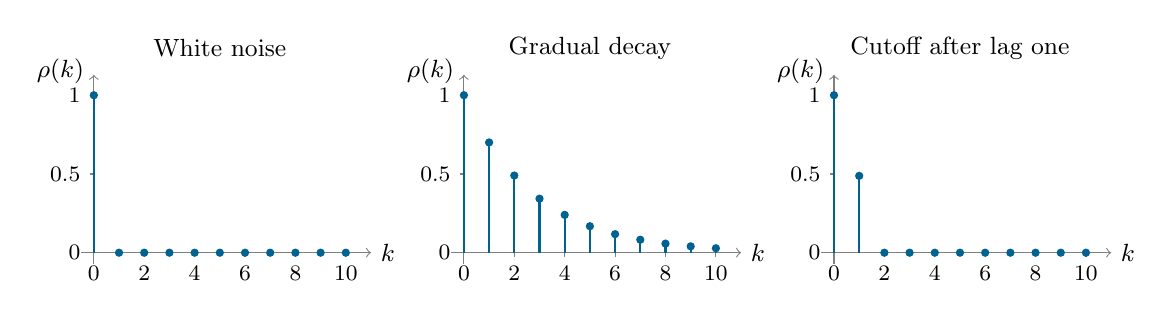
\begin{tikzpicture}[x=0.32cm,y=2cm,font=\small]
	\foreach \panel/\heading in {0/White noise,1/Gradual decay,2/Cutoff after lag one} {
		\begin{scope}[xshift=\panel*4.7cm]
			\node at (5,1.3) {\heading};
			\draw[->,gray] (-0.5,0) -- (11,0) node[right,black] {$k$};
			\draw[->,gray] (0,-0.07) -- (0,1.13);
			\node[left] at (0,1.15) {$\rho(k)$};
			\foreach \y in {0,0.5,1} {
				\draw[gray] (-0.15,\y) -- (0,\y);
				\node[left] at (-0.15,\y) {\footnotesize $\y$};
			}
			\foreach \k in {0,2,4,6,8,10} {
				\draw[gray] (\k,0) -- (\k,-0.025);
				\node[below] at (\k,-0.025) {\footnotesize $\k$};
			}
			\foreach \k in {0,...,10} {
				\ifnum\panel=0
					\pgfmathsetmacro{\acfvalue}{ifthenelse(\k==0,1,0)}
				\else\ifnum\panel=1
					\pgfmathsetmacro{\acfvalue}{pow(0.7,\k)}
				\else
					\pgfmathsetmacro{\acfvalue}{ifthenelse(\k==0,1,ifthenelse(\k==1,0.8/1.64,0))}
				\fi\fi
				\draw[myblue,thick] (\k,0) -- (\k,\acfvalue);
				\fill[myblue] (\k,\acfvalue) circle[radius=1.5pt];
			}
		\end{scope}
	}
\end{tikzpicture}
\end{document}
